\documentclass{article}    

\usepackage{graphicx}

\begin{document}

% ------------------------------------------ figure 5

\begin{figure}[!ht] \centering
  \begin{tabular}{cc}
    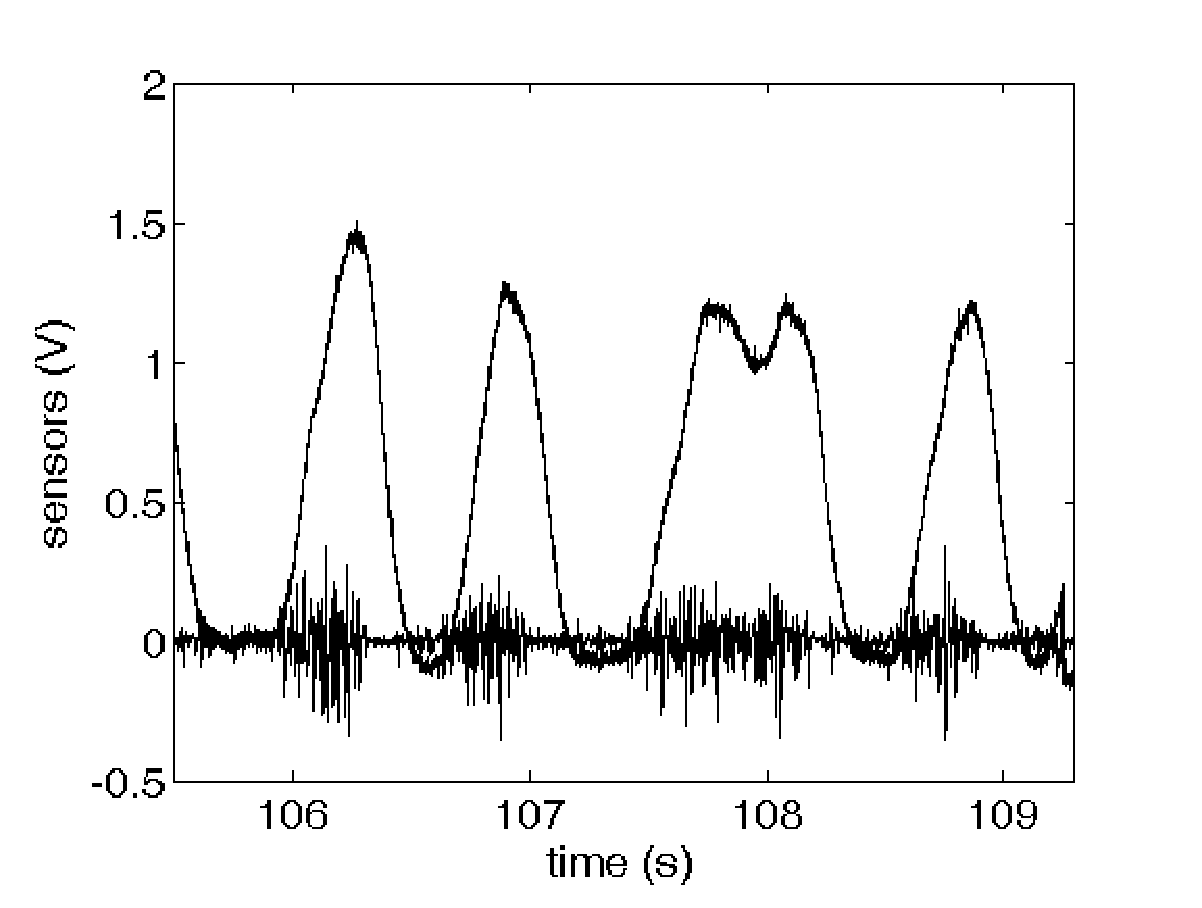
\includegraphics[width=0.50\textwidth]{force_raw.eps} &
    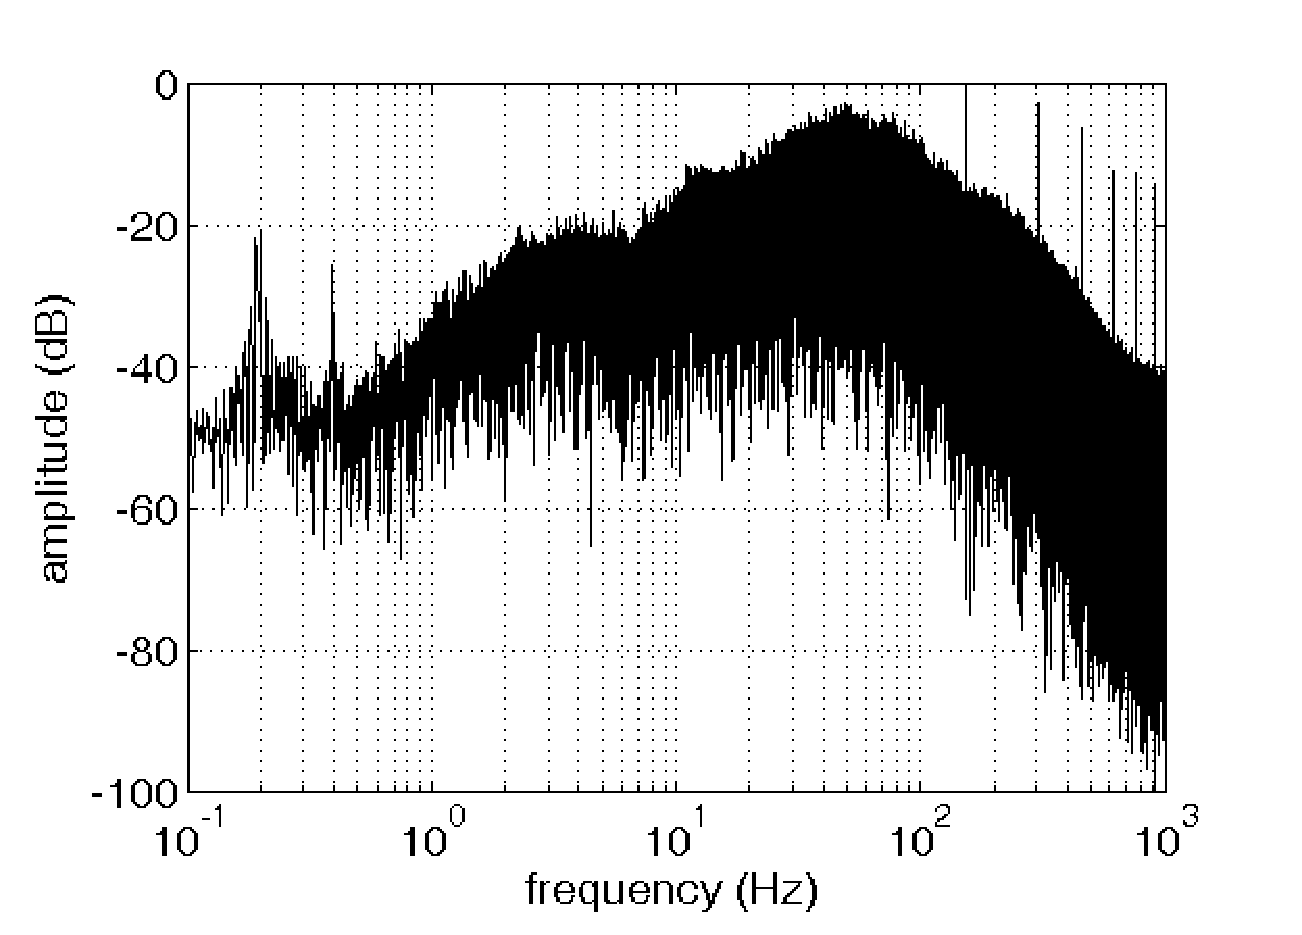
\includegraphics[width=0.50\textwidth]{spectrum_raw.eps} \\
    $(a)$ & $(b)$ \\
  \end{tabular}
%  \caption{$(a)$ typical raw EMG and force signals (the EMG signal
%    being the bottom, high-frequency one); $(b)$ frequency diagram of
%    the EMG signal.}
%  \label{fig:spectra}
\end{figure}

\end{document}
